%%%%%%%%%%%%%%%%%%%%%%%%%%%%%%%%%%%%%%%%%%%%%%%%%%%%%
%
%   Copyright (C), 2016        
%   FILE RUN: CV-JMQ.tex
%
%   RESUME into Latex of Juan Quintana <https://jmquintana79.github.io/>
%
%   AUTHOR: <juan.armaguedon@gmail.com>
%   CREATION DATE: 2016-03-21
%   LAST MODIFIED DATE: 2016-03-21
%   VERSION: v0
%   HELP:
%   - Vocals with accents: � = á; � = é; � = í; � = ó
%
%%%%%%%%%%%%%%%%%%%%%%%%%%%%%%%%%%%%%%%%%%%%%%%%%%%%%

% resume.tex
% vim:set ft=tex spell:

%\documentclass[10pt,letterpaper]{article}

\documentclass[9pt,letterpaper]{extreport}
\usepackage[letterpaper,margin=0.75in]{geometry}
\usepackage[utf8]{inputenc}
\usepackage{mdwlist}
\usepackage[T1]{fontenc}
\usepackage{textcomp}
\usepackage{tgpagella}
\usepackage{fancyhdr}
%\pagestyle{empty} % Without header and footer
% para incluir foto
\usepackage{graphicx}
% icons
\usepackage{marvosym}
\usepackage{ fancyhdr }
\usepackage{ifsym} 
%color
\usepackage{color}
\usepackage[dvipsnames]{xcolor}
\usepackage{pstricks}

    
    

% Format header and footer
\pagestyle{fancyplain}
\renewcommand{\headrulewidth}{0pt}  % Delete line of the header

\lhead{}
\chead{}
\rhead{}
\lfoot{}
\cfoot{}
\rfoot{Mar 2016}				% Rigth footer. Other one on blank.

\setlength{\tabcolsep}{0em}

% indentsection style, used for sections that aren't already in lists
% that need indentation to the level of all text in the document
\newenvironment{indentsection}[1]%
{\begin{list}{}%
	{\setlength{\leftmargin}{#1}}%
	\item[]%
}
{\end{list}}

% opposite of above; bump a section back toward the left margin
\newenvironment{unindentsection}[1]%
{\begin{list}{}%
	{\setlength{\leftmargin}{-0.5#1}}%
	\item[]%
}
{\end{list}}

% format two pieces of text, one left aligned and one right aligned
\newcommand{\headerrow}[2]
{\begin{tabular*}{\linewidth}{l@{\extracolsep{\fill}}r}
	#1 &
	#2 \\
\end{tabular*}}

% make "C++" look pretty when used in text by touching up the plus signs
\newcommand{\CPP}
{C\nolinebreak[4]\hspace{-.05em}\raisebox{.22ex}{\footnotesize\bf ++}}


% define tabuladores
%\newcommand{\itab}[1]{\hspace{0em}\rlap{#1}}
\newcommand{\tab}[1]{\hspace{.4\textwidth}\rlap{#1}}
\newcommand{\tabl}[1]{\hspace{.6\textwidth}\rlap{#1}}
\newcommand{\tabm}[1]{\hspace{.5\textwidth}\rlap{#1}}


% and the actual content starts here
%*******************************************************************

\begin{document}


% HEADER
%*******************************************************************

\begin{minipage}{0.50\textwidth}
\begingroup

%%% LEFT COLUMN 
%\begin{center}
%\Huge \textbf{Juan M. Quintana}
   \fontsize{26pt}{20pt}\fontfamily{lmss}\selectfont \textbf{Juan Quintana} 


%\end{center}

\endgroup
\end{minipage}
\begin{minipage}{0.3\textwidth}

\begin{flushright}
% Address
\textcolor{NavyBlue}{{\textifsymbol{19} Osaka, Japan}}

% Telephone number
\textcolor{NavyBlue}{\Mobilefone{ +8109098889027}}

% Mail
\textcolor{NavyBlue}{\Email{ jmq.veguillas@gmail.com}}


\end{flushright}
\end{minipage}
\begin{minipage}{0.15\textwidth}
%\flushright{\rule{3.5cm}{4.5cm}}
\flushright{\fbox{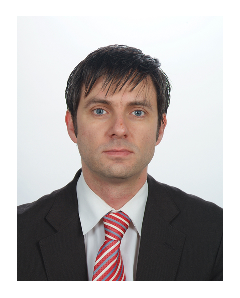
\includegraphics[width=2cm]{img/cv-photo_low_quality.eps}}}
\end{minipage}
\\



% FIRST SECTION
%*******************************************************************
%\hrule
\vspace{-1em} % Include vertical space
\subsection*{\textcolor{NavyBlue}{ \fontsize{12pt}{20pt}\fontfamily{lmss}\selectfont \textbf{WORKING EXPERIENCE} }}


\begin{itemize}
	\parskip=0.1em


% SIXTH EMPLOYMENT
	\item[$\cdot$]
	\headerrow
		{\textbf{Japan Meteorological Corporation}}
		{\textbf{Osaka, Japan}}
	\\
	\headerrow
		{\emph{Research and Development Department Manager: Meteorological Technician \& Senior Developer}}
		{\emph{2015 -- currently}}
	\begin{itemize*}
		\item CFD models: WindSim, WAsP and Phoenics
		\item Datamining to study patterns of apps use in Japan
		\item Web data scraping and analysis of contamination spread
		\item Analysis of weather application content and customer preferences in Japan
		\item Setup Galion Doppler Lidar device
		\item Wind Offshore exhibitor staff in WIND EXPO 2016 
		\item Development of environmental software
	\end{itemize*}


% FIFTH EMPLOYMENT
	\item[$\cdot$]
	\headerrow
		{\textbf{EREDA, Renewable Energy Solutions}}
		{\textbf{Madrid, Spain}}
	\\
	\headerrow
		{\emph{Research and Development Department Manager: Meteorological Technician \& Senior Developer}}
		{\emph{2012 -- 2015}}
	\begin{itemize*}
		\item Solar and meteorological (WRF) modelling.
		\item Data processing and statistical analysis software development.
		\item Management, design, development, testing and server implementation of web application.
		\item Technical and functional analysis of software projects.
	\end{itemize*}


% FOURTH EMPLOYMENT
	\item[$\cdot$]
	\headerrow
		{\textbf{Foundation for Research of Climate Change (FIC) and Meteogrid}}
		{\textbf{Madrid, Spain}}
	\\
	\headerrow
		{\emph{Meteorological Technician \& Software Developer}}
		{\emph{2010 -- 2012}}
	\begin{itemize*}
		\item Use, development and validation of  statistical downscaling technique for climate forecast.	
		\item Local and synoptic subjective weather conditions forecast in Spain.
		\item Preparing weather and climatic reports in different places of the world.
		\item Technical contributions in scientific poster.		
		\item Management and processing of massive datasets.
	\end{itemize*}

% THIRD EMPLOYMENT
	\item[$\cdot$]
	\headerrow
		{\textbf{Spain Meteorological Agency (AEMET)}}
		{\textbf{Málaga, Spain}}
	\\
	\headerrow
		{\emph{Aeronautic meteorological observer }}
		{\emph{2010}}
	\begin{itemize*}
		\item Government employee in Prediction and Monitoring Group of Andalucia, Spain.
		\item Support of meteorologist and meteorological monitoring. 
	\end{itemize*}

% SECOND EMPLOYMENT
	\item[$\cdot$]
	\headerrow
		{\textbf{Spain Meteorological Agency (AEMET)}}
		{\textbf{Madrid, Spain}}
	\\
	\headerrow
		{\emph{Fellow graduate}}
		{\emph{2007 -- 2009}}
	\begin{itemize*}
		\item Project ENSEMBLES:  "Application of dynamic techniques of downscaling for seasonal forecast".
		\item European Centre for Medium-Range Weather Forecast (ECMWF) supercomputer use. 
		\item Working with numerical models for seasonal forecast.
	\end{itemize*}

% FIRST EMPLOYMENT
	\item[$\cdot$]
	\headerrow
		{\textbf{CORITEL SA (Accenture Spain)}}
		{\textbf{Madrid, Spain}}
	\\
	\headerrow
		{\emph{Junior Programmer}}
		{\emph{2006 -- 2007}}
	\begin{itemize*}
		\item Lotus Notes environment: errors control, technical and functional analysis.
	\end{itemize*}
\end{itemize}


% SECOND SECTION
%*******************************************************************
%\hrule
\vspace{-1em}
\subsection*{\textcolor{NavyBlue}{ \fontsize{12pt}{20pt}\fontfamily{lmss}\selectfont \textbf{EDUCATION} }}



\begin{itemize}
	\parskip=0.1em

% SIXTH EDUCATION
	\item[$\cdot$] 
	\headerrow
		{\textbf{College course in Satellite Remote Sensing : 800 hours}}
		{\textbf{Distance course}}
	\\
	\headerrow
		{\emph{Spanish Distance Learning College (UNED)}}
		{\emph{2009 -- 2010}}

% FITH EDUCATION
	\item[$\cdot$]
	\headerrow
		{\textbf{Aeronautic meteorological observer course: 120 hours}}
		{\textbf{Madrid, Spain}}
	\\
	\headerrow
		{\emph{Spain Meteorological Agency (AEMET)}}
		{\emph{2009}}
	
% FOURTH EDUCATION
    \item[$\cdot$] 
    \headerrow
    	{\textbf{Training course in Junior Programmer: 320 hours}}
		{\textbf{Madrid, Spain}}
	\\
	\headerrow
		{\emph{Coritel SA (Accenture Spain)}}
		{\emph{2006}}
	
% THIRD EDUCATION
%	\item 
%	\headerrow
%		{\textbf{Degree in Mathematical (only five subjects)}}
%		{\textbf{Distance course}}
%	\\
%	\headerrow
%		{\emph{Spanish Distance Learning College (UNED)}}
%		{\emph{2005 -- 2006}}
	
% SECOND EDUCATION
	\item[$\cdot$] 
	\headerrow
		{\textbf{Course: "Programming languages": 309 hours / C, \CPP y Visual \CPP}}
		{\textbf{Guadalajara, Spain}}
	\\
	\headerrow
		{\emph{CEI \& Languages Academy }}
		{\emph{2005}}
	
% FIRSTH EDUCATION
	\item[$\cdot$] 
	\headerrow
		{\textbf{Degree in Physics: applied physics option}}
		{\textbf{Madrid, Spain}}
	\\
	\headerrow
		{\emph{Universidad Autónoma de Madrid (UAM)}}
		{\emph{1999 -- 2004}}
		
\end{itemize}



% THIRD SECTION
%*******************************************************************
%\hrule
\vspace{-1em}
\subsection*{\textcolor{NavyBlue}{ \fontsize{12pt}{20pt}\fontfamily{lmss}\selectfont \textbf{MAIN TECHNICAL SKILLS} }}


\begin{indentsection}{\parindent}
\hyphenpenalty=1000

\begin{description*}
% Programming languages
	\item[$\cdot$  Programming languages:]
	Fortran, Shell-Script, AWK, R, MatLab, Lotus Notes, C, \CPP, OpenMP, Visual C++, Visual Basic, Python, Numpy, Pandas, Scipy, Git, Java, Java-Script, jQuery, Angular JS, SQL, HTML, CSS, \LaTeX, PHP, Apache
	\item[$\cdot$  OS:]
	Linux (Ubuntu, Debian, CentOS, Redhat), Mac OS X, Windows
	\item[$\cdot$  Languages:]
	ENGLISH - B1 TOEIC $\ast$ SPANISH - MOTHER LANGUAGE $\ast$ Studying Japanese
	\end{description*}

\end{indentsection}

% FOURTH SECTION
%*******************************************************************
%\hrule
\vspace{-1em}
\subsection*{\textcolor{NavyBlue}{ \fontsize{12pt}{20pt}\fontfamily{lmss}\selectfont \textbf{OBJECTIVE STATEMENTS} }}


\begin{indentsection}{\parindent}
	Begin a professional career in Japan $\ast$ Learn Japanese language $\ast$ Live in Japan for a long time.
\end{indentsection}	

% FIFTH SECTION
%*******************************************************************
%\hrule
\vspace{-0.4em} % Include vertical space

\subsection*{\textcolor{NavyBlue}{ \fontsize{12pt}{20pt}\fontfamily{lmss}\selectfont \textbf{ANNEX - EVOLUTION OF TECHNICAL KNOWLEDGE} }}



\begin{itemize}
	\parskip=0.1em

% PERSONAL IMPROVEMENT
	\item[$\cdot$]
	\headerrow
		{\textbf{Skills developed outside work }}
		{\textbf{Currently}}
	\begin{itemize*}
	    % Language 1
		\item 
		\headerrow
			{\textbf{Python}} 
			{\emph{Advanced Level}}
			\\			
		    Algorithms development: data web parsing, data processing and analysis -> DATA MINING.
			\\			
		    Frameworks Numpy, Pandas and Scipy use.
			\\
			Web API for Python: Evernote, Twitter, Lindekin.
			\\			
		    Python Web Framework: Bottle. 		    
	    % Language 2
		\item 
		\headerrow
			{\textbf{R, MatLab}} 
			{\emph{Advanced Level}}
			\\			
		    Meteorological and climatic data mining and statistical analysis.
	    % Language 3
		\item 
		\headerrow
			{\textbf{\LaTeX}} 
			{\emph{Medium Level}}
			\\			
		    Technical and personal  templates/documents creation.	    
	    % Language 4
		\item 
		\headerrow
			{\textbf{PHP, HTML, CSS, Javascript}} 
			{\emph{Advanced Level}}
			\\			
		    Websites creation, maintenance and management. Data web parsing. 
	    % Language 5
		\item 
		\headerrow
			{\textbf{LINUX / Shell-Script}} 
			{\emph{Advanced Level}}
			\\
		    Scripts development to process and manage datasets.
		    \\
		    Root account using of operative system based in Linux / Unix (Ubuntu, Debian, Mac OS X).				
		 
	\end{itemize*}


% FOURTH EMPLOYMENT
	\item[$\cdot$]
	\headerrow
		{\textbf{EREDA, Renewable Energy Solutions}}
		{\textbf{2012 -- currently}}
	\begin{itemize*}
	    % Lenguage 1
		\item 
		\headerrow
			{\textbf{Project management and software development}} 
			{\emph{Medium Level}}
			\\			
		    Consultant in Windows 8 desktop app development project. 
			\\					    
		    Technical and functional manager of web application development platform for visual and\\ statistical data analysis made in Django framework. 
	    % Lenguage 2
		\item 
		\headerrow
			{\textbf{Hardware and software management of company}} 
			{\emph{Medium Level}}
			\\			
		    Linux web server installation and management.
			\\
		    Networks management and monitoring.
			\\
		    Computers and information systems management.
	         % Lenguage 3
		\item 		
		\headerrow
			{\textbf{Python, Object Oriented Programming }} 
			{\emph{Advanced Level}}
			\\			
		    Modeling, data proccesing.
			\\		    
		    Django project (backend) design and development.
	         % Lenguage 4
		\item 		
		\headerrow
			{\textbf{MySQL}} 
			{\emph{Advanced Level}}
			\\			
		    Management and data processing.
			\\
		    Django project (backend) development.
			\\
		    Data storage and backup systems development of company.		    

	         % Lenguage 5
		\item 		
		\headerrow
			{\textbf{HTML, CSS, Javascript, javascript frameworks: jQuery, Angular JS }} 
			{\emph{Medium-Advanced Level}}
		    Django project (client side) design and development.


	         % Lenguage 6
		\item 
		\headerrow
			{\textbf{C++ , Object Oriented Programming}} 
			{\emph{Medium-Advanced Level}}
			\\			
		    Data processing scripts development written in Object Oriented Programming and in\\ parallel execution programming with OpenMP. 
			\\			
		    Development of solar production algorithm using Object Oriented Programming and \\own libraries. 
		% Lenguage 7    
		\item 
		\headerrow
			{\textbf{LINUX / Shell-Script}} 
			{\emph{Advanced Level}}
			\\			
		    Data processing scripts and jobs development.
		    Ubuntu OS user with root account.
		% Lenguage 8
		\item 		
		\headerrow
			{\textbf{R y Matlab}} 
			{\emph{Advanced Level}}
			\\			
		    Modeling, data statistical analysis and plotting in R environment.
		% Lenguage 9
		\item 		
		\headerrow
			{\textbf{CDO, XConv, GRIBEX, Ferret, etc}} 
			{\emph{Medium Level}}
			\\			
			Use and development with command scripting to  process and manage binary data (GRIB and\\ NETCDF format).		
		% Lenguage 10
		\item 
		\headerrow
			{\textbf{FORTRAN}} 
			{\emph{Advanced Level}}
			\\			
		    Modeling and data processing. 
	\end{itemize*}




% THIRD EMPLOYMENT
	\item[$\cdot$]
	\headerrow
		{\textbf{Foundation for Research of Climate Change (abbreviation into spanish, FIC) and Meteogrid}}
		{\textbf{2010 -- 2012}}
	\begin{itemize*}
	    % Lenguage 1
		\item 
		\headerrow
			{\textbf{FORTRAN}} 
			{\emph{Advanced Level}}
			\\			
		    Modeling with statistical algorithm, heavy computations and data processing.
		% Lenguage 2    
		\item 
		\headerrow
			{\textbf{LINUX / Shell-Script}} 
			{\emph{Medium Level}}
			\\			
		    Data processing scripts and jobs development.
		    Ubuntu OS user with root account.
		% Lenguage 3
		\item 		
		\headerrow
			{\textbf{R}} 
			{\emph{Basic Level}}
			\\			
		    Modeling, data statistical analysis and plotting in R environment.
		% Lenguage 4
		\item 		
		\headerrow
			{\textbf{Python}} 
			{\emph{Basic Level}}
			\\			
		    Data processing and web parsing.
		% Lenguage 5
		\item 		
		\headerrow
			{\textbf{CDO, GRIBEX, Ferret, etc}} 
			{\emph{Basic Level}}
			\\			
			Use and development with command scripting to  process and manage binary data (GRIB and\\ NETCDF format).		    
	\end{itemize*}
% SECOND EMPLOYMENT
    % No progamming.

% SECOND EMPLOYMENT
	\item[$\cdot$]
	\headerrow
		{\textbf{Agencia Estatal de Meteorología (AEMET)}}
		{\textbf{2007 -- 2009}}
	\begin{itemize*}
	    % Lenguage 1
		\item 
		\headerrow
			{\textbf{FORTRAN}} 
			{\emph{Medium-Advanced Level}}
			\\			
		     Modeling with dynamical algorithm, heavy computations and data processing.
		% Lenguage 2    
		\item 
		\headerrow
			{\textbf{LINUX / Shell-Script y AWK}} 
			{\emph{Medium Level}}
			\\			
		    Data processing scripts and remote jobs development.
		    RedHat OS user with root account.

		% Lenguage 3
		\item 		
		\headerrow
			{\textbf{Metview, CDO, GRIBEX, Ferret, etc}} 
			{\emph{Basic Level}}
			\\			
			Use and development with command scripting to  process and manage binary data (GRIB and\\ NETCDF format).		    
	\end{itemize*}

% FIRST EMPLOYMENT
	\item[$\cdot$]
	\headerrow
		{\textbf{CORITEL SA (Accenture Spain)}}
		{\textbf{2006 -- 2007}}
	\begin{itemize*}
	    % Lenguage 1
		\item 
		\headerrow
			{\textbf{LOTUS NOTES}} 
			{\emph{Medium-Advanced Level}}
			\\			
		    Maintenance and development: errors control, software and databases technical and\\ functional analysis.
	    % Lenguage 2
		\item 
		\headerrow
			{\textbf{Java (Education)}} 
			{\emph{Basic Level}}
			\\			
		    Java education during 3 weeks in company: basic Object Oriented Programming and background\\ running by {\emph{pipes}}. 
	    % Lenguage 3
		\item 
		\headerrow
			{\textbf{JavaScript, HTML, SQL, ASP (Education)}} 
			{\emph{Basic Level}}
			\\			
		    Basic education during 2 weeks in company. 
	    % Lenguage 4
		\item 
		\headerrow
			{\textbf{Visual Basic (Education)}} 
			{\emph{Basic Level}}
			\\			
		    Education during 1 month and practise programming a  Windows desktop application with web\\ interaction. 	    
	\end{itemize*}

% COMPLEMENTARY EDUCATION
	\item[$\cdot$]
	\headerrow
		{\textbf{EDUCATION: Course "Programming languages"}}
		{\textbf{2005}}
	\begin{itemize*}
	    % Lenguage 1
		\item 
		\headerrow
			{\textbf{C, \CPP  y Visual \CPP  (Education)}} 
			{\emph{Basic-Medium Level}}
			\\			
		    Course during 309 hours and practise programming a  Windows desktop financial management \\software.
		    
	\end{itemize*}
\end{itemize}

%\rfoot{Julio 2012}

\end{document}
%**************************************************************
